\clearpage
\section{Sanctuary Places and Furnishings}
\PCDPlateHeader{Plate II --- Principal Sanctuary Furnishings}{Not to common scale}
\ifdefined\TriptychPrintEdition
\begin{center}
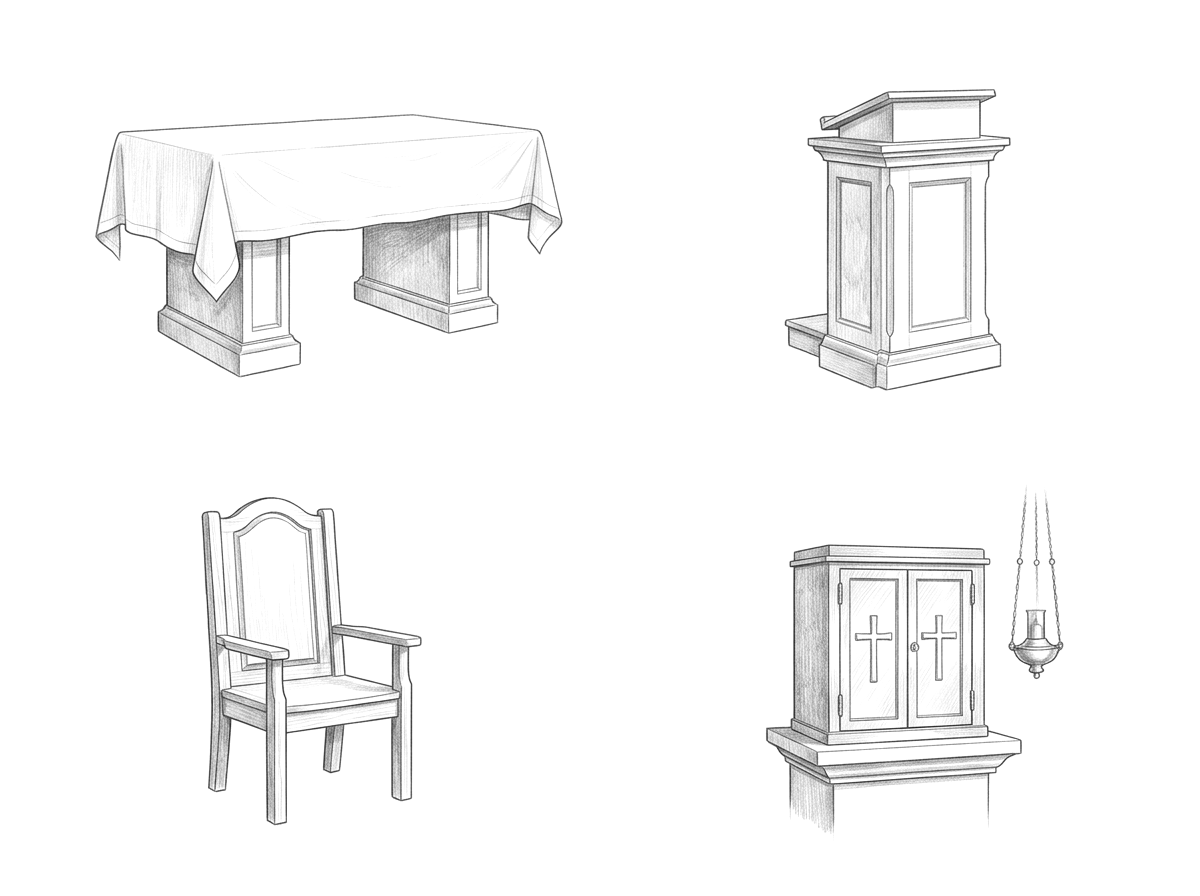
\includegraphics[width=0.92\linewidth,height=3.55in,keepaspectratio]{liturgy/roman-rite/postconciliar/2008-latin-2011-us-english/reference/roman-sanctuary-dictionary/shared/artwork/graphite/pc-art-02-altar-ambo-chair.png}
\end{center}
\PCDPositionKey{Top left: freestanding Altar covered with white linen cloth; top right: stationary stone Ambo with sloped desk and step; bottom left: dignified wooden Presidential Chair; bottom right: locked double-door Tabernacle on stone pedestal beside suspended oil Sanctuary Lamp.}
\else
\textbf{Visual Plate Summary (Plate II --- Principal Sanctuary Furnishings, Not to common scale):} Four-subject monochrome graphite architectural study comparing the principal sanctuary furnishings: top left, a freestanding carved stone altar dressed in a white linen altar cloth; top right, a permanent paneled stone ambo with angled book rest and rear step; bottom left, a stately wooden presidential chair with armrests; bottom right, a solid locked double-door metal tabernacle on a stone pedestal with a suspended sanctuary lamp burning beside it.

\textbf{Reading order and object placement:} Top left: freestanding Altar covered with white linen cloth; top right: stationary stone Ambo with sloped desk and step; bottom left: dignified wooden Presidential Chair; bottom right: locked double-door Tabernacle on stone pedestal beside suspended oil Sanctuary Lamp.
\fi

\label{pc-obj-altar}
\PCDEntryHead{Altar}{Altare}{required}{N01}
\PCDField{Also called}{Altar Table; Mensa; \textit{Mensa Domini}; \textit{Altare fixum}; \textit{Altare mobile}}
The freestanding altar at the center of the sanctuary is the sacred table where Christ's sacrifice is offered. Whenever you arrive at or leave the sanctuary during Mass, make a profound bow to the altar (or genuflect if the tabernacle with the Blessed Sacrament stands in the sanctuary, except when carrying the processional cross or lighted candles). At the Preparation of the Gifts, bring the Roman Missal, folded linens, and empty sacred vessels cleanly to the edge of the mensa when no deacon or instituted acolyte does so. Never lean on the altar, leave cruets sitting on the cloth, or kiss the mensa---venerating the altar with a kiss belongs to the bishop, priest, and deacon.

\PCDField{Where to look on the plate}{Top left (Plate II); center (Plate I)}
\PCDField{Handling boundary}{\textbf{Server recognizes only; does not handle.} Servers venerate the altar with a profound bow on approaching or departing (genuflecting instead if the Blessed Sacrament is reserved in the sanctuary), place the Roman Missal and unconsecrated vessels upon it at the Preparation of the Gifts when needed, and never lean upon, clutter, or kiss the mensa (kissing the altar belongs to the bishop, priest, and deacon). (Ordinary ministers: Bishop, Priest, Deacon.)}
\PCDSafety{Keep the altar table clear of spare papers, cruets, and extraneous items (GIRM 306), guard against candle flames and dripping wax near the white cloth, and notify the priest or deacon immediately if any Precious Blood is spilled---never attempt to blot or wash a spill yourself (GIRM 280).}
\PCDField{Do not confuse with}{Credence Table}
\PCDEntryRule

\label{pc-obj-ambo}
\PCDEntryHead{Ambo}{Ambo}{required}{N02}
\PCDField{Also called}{Lectern of the Word; \textit{Lectrinum}}
The permanent stone or wood ambo stands toward the front of the sanctuary for the Liturgy of the Word. Before Mass, you may check that the Lectionary is open to the right page on its sloped desk, and during the Gospel procession you walk ahead with lighted candles or the thurible and stand neatly beside the ambo facing the deacon or priest. Keep an eye on the step behind the ambo when carrying lighted candles, and remember that altar servers do not read from the ambo unless separately scheduled as readers.

\PCDField{Where to look on the plate}{Top right (Plate II); left foreground (Plate I)}
\PCDField{Handling boundary}{\textbf{Server recognizes only; does not handle.} Servers flank the ambo with lighted candles and incense during the Gospel proclamation and may confirm before Mass that the Lectionary rests open upon the desk, but never proclaim readings or lead prayers from the ambo unless separately deputed as readers. (Ordinary ministers: Bishop, Priest, Deacon, Instituted lector.)}
\PCDSafety{Watch the rear step of the ambo when moving into place with lighted Gospel candles or a smoking thurible, keeping flames well clear of the microphone, Lectionary pages, and ministers' vestments.}
\PCDField{Do not confuse with}{Missal Stand}
\PCDEntryRule

\label{pc-obj-presidential-chair}
\PCDEntryHead{Presidential Chair}{Sedes sacerdotis celebrantis}{required}{N03}
\PCDField{Also called}{Chair for the Priest Celebrant; Presider's Chair; \textit{Sedes}}
The stately single wooden armchair in the sanctuary belongs exclusively to the presiding priest---servers never sit in it, even before or after Mass. Your main job here as book-bearer is to step cleanly beside or in front of the priest when he stands for the Collect, the conclusion of the Prayer of the Faithful, and the Prayer after Communion, holding the Roman Missal or the lighter Book of the Chair steady at a comfortable reading angle without blocking his view of the congregation.

\PCDField{Where to look on the plate}{Bottom left (Plate II); rear right (Plate I)}
\PCDField{Handling boundary}{\textbf{Clergy-reserved; server does not touch.} Reserved strictly to the priest celebrant (or bishop when celebrating outside his cathedral); altar servers never sit in the presidential chair and approach it solely to hold the Roman Missal or Book of the Chair during prayers. (Ordinary ministers: Priest, Bishop.)}
\PCDEntryRule

\label{pc-obj-credence-table}
\PCDEntryHead{Credence Table}{Abacus}{required}{N04}
\PCDField{Also called}{Side Table; Credence; \textit{Credentia}; \textit{Mensa credentiae}}
Think of the credence table at the side of the sanctuary as your staging station during Mass. Before the procession, check that the unconsecrated chalice, folded linens, cruets, lavabo pitcher, basin, towel, and Communion-plate are arranged neatly with room to work. At the Preparation of the Gifts, bring the vessels, linens, cruets, and lavabo smoothly to the altar and return empty cruets right back to the credence table so nothing crowds the altar cloth. After Communion, bring the water cruet if asked, but never touch or wash any unpurified vessel resting on a corporal.

\PCDField{Where to look on the plate}{See Plate I, far right beside the presidential chair}
\PCDField{Handling boundary}{\textbf{Server prepares or sets in place before or during Mass.} Servers help arrange clean unconsecrated vessels, linens, cruets, and lavabo equipment on the credence table before Mass, carry needed items to the altar at the Preparation of the Gifts, and bring the water cruet for purification without touching unpurified sacred vessels. (Ordinary ministers: Priest, Deacon, Instituted acolyte.)}
\PCDSafety{After Communion, never purify sacred vessels at the credence table and never disturb unpurified vessels left suitably covered upon a corporal there; purification belongs strictly to the priest, deacon, or instituted acolyte (GIRM 279; Redemptionis Sacramentum 119; USCCB Norms 53).}
\PCDField{Do not confuse with}{Altar}
\PCDEntryRule

\label{pc-obj-tabernacle}
\PCDEntryHead{Tabernacle}{Tabernaculum}{required}{N05}
\PCDField{Also called}{Eucharistic Tabernacle}
Inside the locked tabernacle rests the Body of Christ Himself. Whenever the sanctuary lamp burns beside it, genuflect smoothly on your right knee when passing before it outside Mass and at the entrance and exit of Mass when it stands in the sanctuary (unless you are carrying the processional cross or lighted candles, GIRM 274). An altar server never opens the tabernacle, never takes or holds the tabernacle key, and never reaches inside---only clergy, or instituted acolytes and duly mandated extraordinary ministers for Communion, handle what is reserved there.

\PCDField{Where to look on the plate}{Bottom right (Plate II); recessed rear niche (Plate I)}
\PCDField{Handling boundary}{\textbf{Clergy-reserved; server does not touch.} Strictly reserved to clergy (and to instituted acolytes or duly deputed extraordinary ministers solely for Communion distribution or reposition); altar servers never open the tabernacle, handle its key, or touch reserved vessels, and genuflect before it outside Mass and at the beginning and end of Mass when it stands in the sanctuary (GIRM 274). (Ordinary ministers: Bishop, Priest, Deacon.)}
\PCDSafety{Never open the tabernacle, touch the tabernacle key, or retrieve or repose the Blessed Sacrament. Key custody belongs strictly to the pastor or rector (CIC can. 938 §5). Genuflect on the right knee before the tabernacle outside Mass and at the beginning and end of Mass when it stands in the sanctuary (GIRM 274).}
\PCDEntryRule

\label{pc-obj-sanctuary-lamp}
\PCDEntryHead{Sanctuary Lamp}{Lampas peculiaris}{required}{N06}
\PCDField{Also called}{Tabernacle Lamp; Presence Lamp; \textit{Lampas sanctuarii}; \textit{Lucerna}}
Whenever you enter the sanctuary, glance first toward the hanging sanctuary lamp beside the tabernacle. Its steady living flame tells you immediately that the Blessed Sacrament is reserved inside, signaling when to genuflect before the tabernacle. Servers never light, extinguish, or touch the sanctuary lamp during Mass; if the sacristan asks for help replenishing it outside Mass, handle hot glass and open flame with patience and care.

\PCDField{Where to look on the plate}{Suspended beside the tabernacle at bottom right (Plate II) and in the rear niche (Plate I)}
\PCDField{Handling boundary}{\textbf{Server recognizes only; does not handle.} Servers look to the burning sanctuary lamp as the unmistakable sign that Christ is reserved in the tabernacle and never light, move, or extinguish it during Mass; any maintenance outside Mass follows sacristan direction with fire-safety care. (Ordinary ministers: Priest, Sacristan.)}
\PCDSafety{Never extinguish, move, or adjust the sanctuary lamp during Mass, and never extinguish it while the Blessed Sacrament remains reserved in the tabernacle. If assisting the sacristan outside Mass to replace a sanctuary candle or oil vessel, allow hot glass and oil to cool safely, guard against open flame, and never open the tabernacle.}
\PCDField{Do not confuse with}{Altar Candles}
\PCDEntryRule

\label{pc-obj-baptismal-font}
\PCDEntryHead{Baptismal Font}{Fons baptismalis}{required}{N07}
\PCDField{Also called}{Font; \textit{Fons baptismatis}}
You will serve around the octagonal baptismal font during parish Baptisms and the Easter Vigil procession. Your role is to accompany the priest or deacon carrying the processional cross, lighted candles, the ritual book, or a clean tray with linen towels and the closed holy-oil stocks when requested. Leave the pouring of water and all anointings to the clergy, watch for slippery droplets on the floor around the basin, and never dump blessed baptismal water down an ordinary drain.

\PCDField{Where to look on the plate}{See Plate X, bottom right}
\PCDField{Handling boundary}{\textbf{Server recognizes only; does not handle.} Servers walk in procession to the font with cross, candles, ritual book, or drying towels during Baptisms and the Easter Vigil, never pouring sacramental water or disposing of blessed baptismal water improperly. (Ordinary ministers: Bishop, Priest, Deacon.)}
\PCDSafety{Never empty blessed baptismal water into an ordinary sink or sewer drain; blessed water must be poured reverently into the sacrarium or directly into clean earth. Wipe any splashed water from stone or tiled steps immediately to prevent slipping.}
\PCDField{Do not confuse with}{Aspergillum and Aspersorium}
\PCDEntryRule
